\section{Вычислительный эксперимент}\label{sec4}

Проводится эксперимент для анализа свойств предложенных методов оценки достаточного размера выборки. Эксперимент состоит из нескольких частей. В первой части рассматриваются оценки достаточного размера выборки в случае, когда достаточный размер выборки не превосходит доступный. Во второй части исследуются результаты, полученные в условиях того, что достаточный размер выборки больше доступного.

\subsection{Достаточный размер выборки не превосходит доступный}

\subsubsection{Сходимость предложенных функций}

Синтетические данные сгенерированы из модели линейной регрессии. Число объектов 1000, число признаков 20. Из данной выборки последовательно удаляется по одному объекту, пока число объектов в подвыборке не станет равно числу признаков. Такой процесс повторяется $B=1000$ раз. В результате для каждого размера выборки $k$ получено значение каждой из функций $D(k)$, $M(k)$, $KL(k)$ и $S(k)$, определенных в Главе~\ref{sec2} (здесь используется логарифм функции правдоподобия). Далее приведен Рис.~\ref{synthetic-regression-functions}, на котором изображены полученные зависимости.

\begin{figure}[h!]
    \centering
    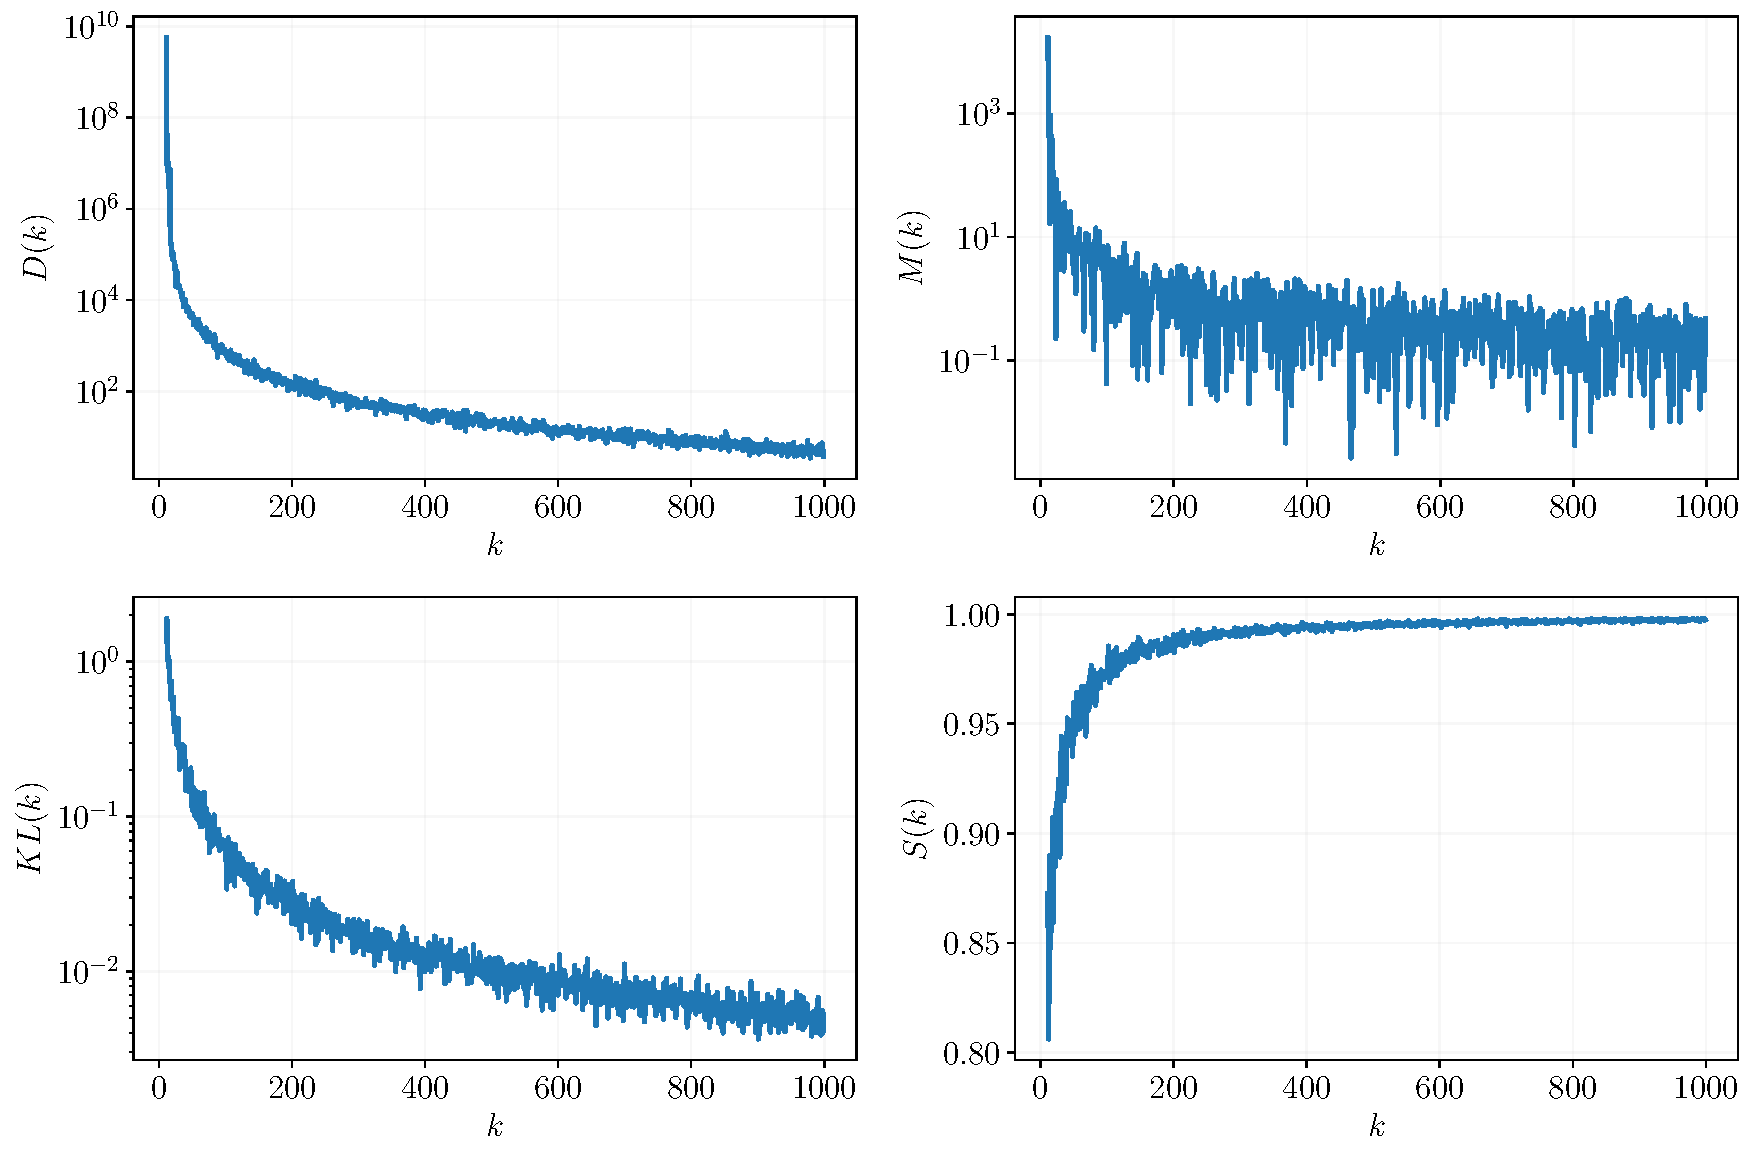
\includegraphics[width=0.9\textwidth]{synthetic-regression-functions}
    \caption{Сходимость функций для синтетической выборки (линейная регрессия)}
    \label{synthetic-regression-functions}
\end{figure}

Полученные графики подтверждают результаты, полученные в Теоремах \ref{theorem1}, \ref{theorem2} и \ref{theorem3}. Значения функций $D(k)$, $M(k)$ и $KL(k)$ стремятся к нулю при увеличении размера подвыборки. Значения $S(k)$ при увеличении размера подвыборки стремятся к единице.

\subsubsection{Определение достаточного размера выборки}

Синтетические данные сгенерированы из модели линейной регрессии. Число объектов 1000, число признаков 20. Далее приведены графики логарифма функции правдоподобия выборки, а также функций $D(k)$ и $M(k)$ для логарифма функции правдоподобия. Использовалось $B=1000$ бутстрап-выборок. Выполнено определение D-достаточного и M-достаточного размеров выборки. Для D-достаточности выбрано $\varepsilon = 3 \cdot 10^{1}$, для M-достаточности $\varepsilon = 4 \cdot 10^{-1}$. Результаты представлены на Рис.~\ref{synthetic-regression-sufficient}. 

\begin{figure}[h!]
    \centering
    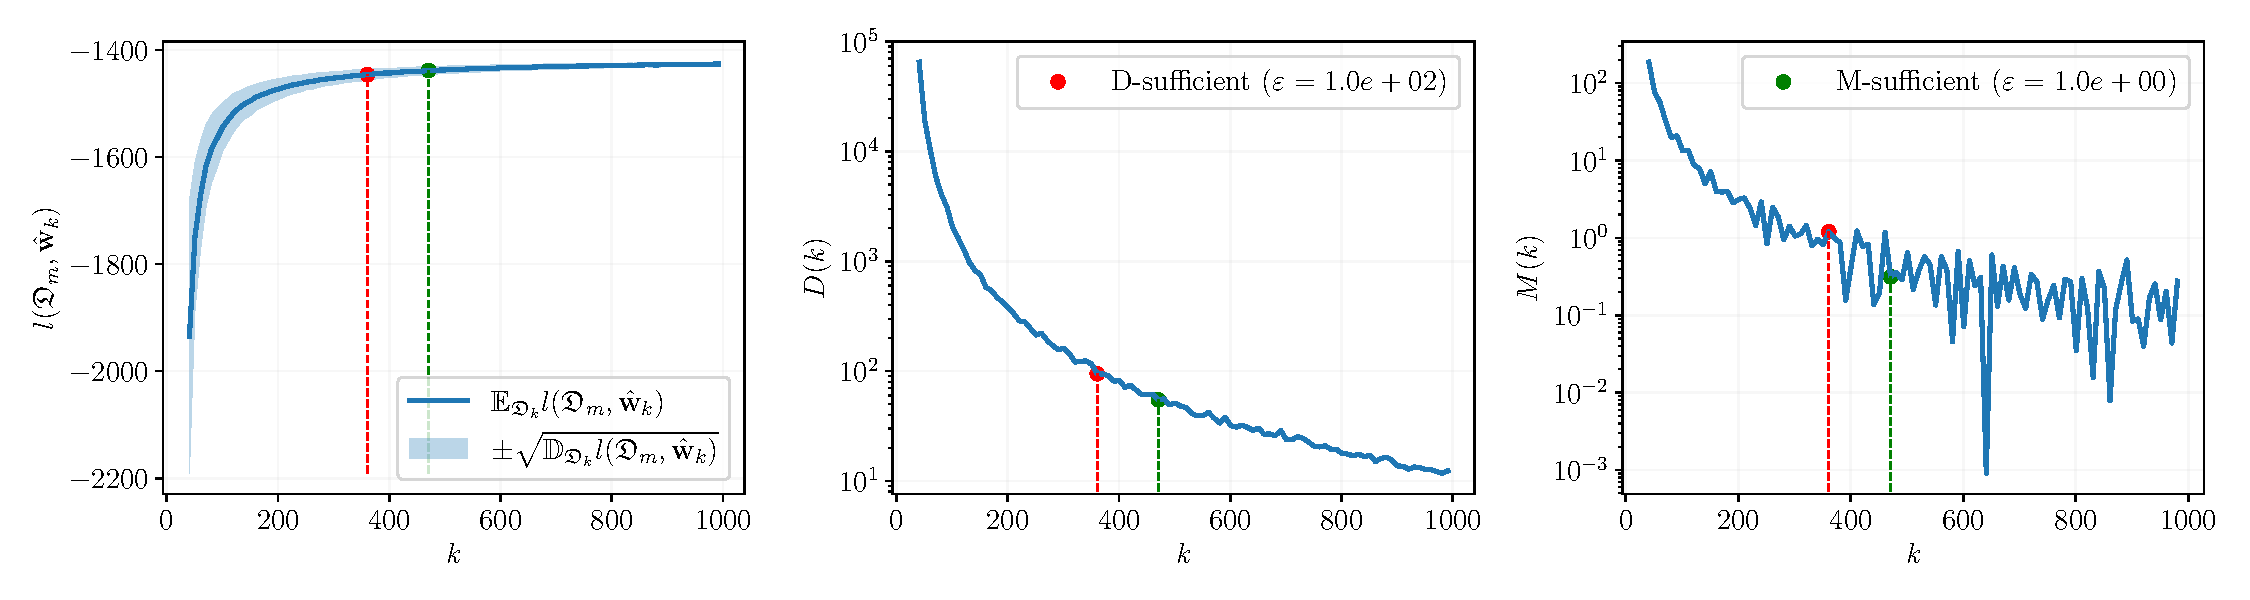
\includegraphics[width=\textwidth]{synthetic-regression-sufficient}
    \caption{Синтетическая выборка (линейная регрессия) при $m^* \leqslant m$}
    \label{synthetic-regression-sufficient}
\end{figure}

Вторая синтетическая выборка сгенерирована из модели логистической регрессии. Число объектов 1000, число признаков 20. Аналогичные графики приведены на Рис.~\ref{synthetic-classification-sufficient}. Для D-достаточности использовалось $\varepsilon = 3 \cdot 10^1$, для M-достаточности $\varepsilon = 6 \cdot 10^{-1}$.

\begin{figure}[h!]
    \centering
    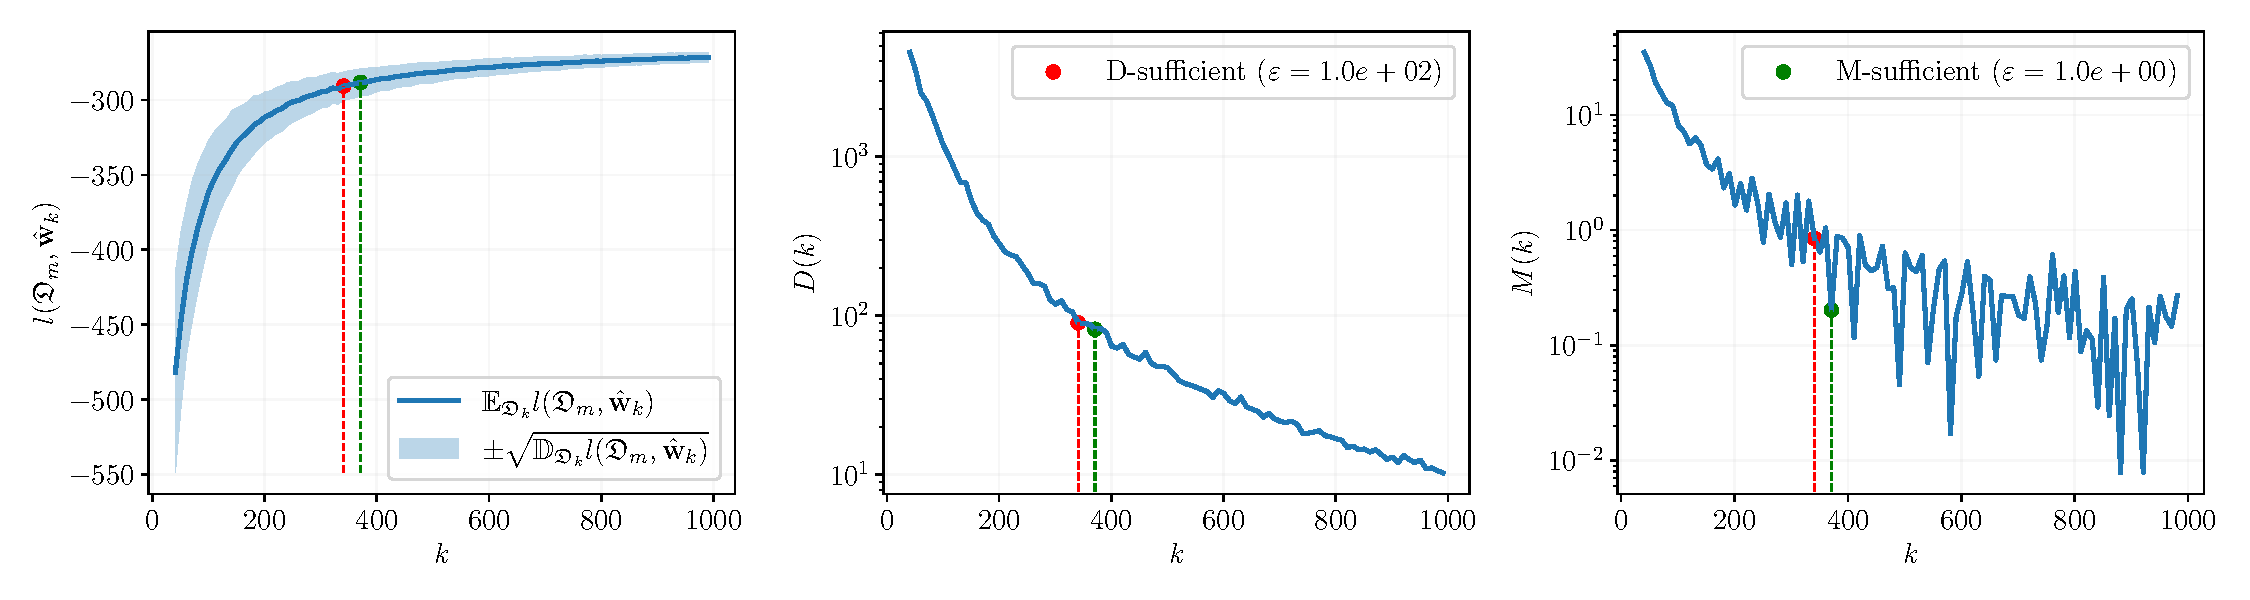
\includegraphics[width=\textwidth]{synthetic-classification-sufficient}
    \caption{Синтетическая выборка (логистическая регрессия) при $m^* \leqslant m$}
    \label{synthetic-classification-sufficient}
\end{figure}

Далее рассматривается пример определения достаточного размера выборки на настоящих данных. Используется датасет Abalone из \citep{UCI} с задачей регрессии. Число объекто 4177, число признаков 8. Полученные результаты на Рис.~\ref{abalone-sufficient}. Определение D-достаточности использует $\varepsilon=2.5 \cdot 10^{-3}$, для M-достаточности взято $\varepsilon=8 \cdot 10^{-3}$.

\begin{figure}[h!]
    \centering
    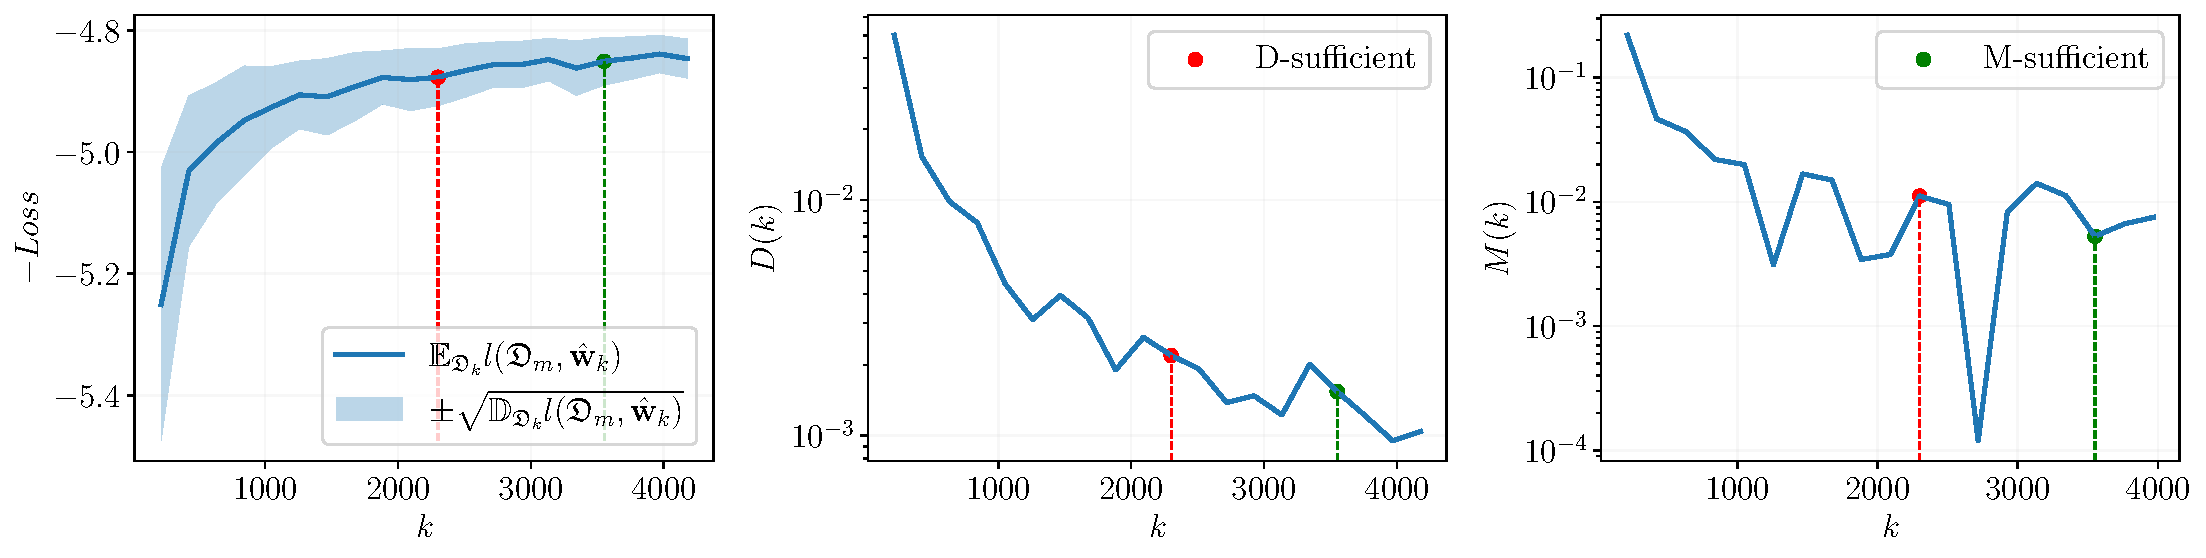
\includegraphics[width=\textwidth]{abalone-sufficient}
    \caption{Выборка Abalone (регрессия) при $m^* \leqslant m$}
    \label{abalone-sufficient}
\end{figure}

\subsection{Достаточный размер выборки больше доступного}

\subsubsection{Определение параметрического семейства функций с помощью генетического алгоритма}

Реализацию генетического алгоритма, приведенного в разделе \ref{ga}, можно найти в \href{https://github.com/kisnikser/Bayesian-Sample-Size-Estimation/tree/main/code/genetic_algorithm}{репозитории}. Для исследования зависимости функции ошибки от используемого размера выборки в задаче регрессии использовались следующие датасеты из \citep{UCI}: Abalone, Auto MPG, Liver Disorders, Wine Quality, Parkinsons Telemonitoring, Bike Sharing Dataset, Real estate valuation и Heart failure clinical records. Была выбрана квадратичная функция потерь MSE. Задача регрессии для каждого из них решалась с помощью линейной регрессии из \citep{scikit-learn}. Усреднение производилось по $B = 100$ бутстрап-выборкам. Как было сказано ранее, все зависимости приводятся к одинаковому масштабу по обеим осям. Полученные графики представлены на Рис.~\ref{datasets-regression}. Слева находится график для выборочного среднего. Справа находится график для выборочного среднеквадратичного отклонения.

\begin{figure}[h!]
    \centering
    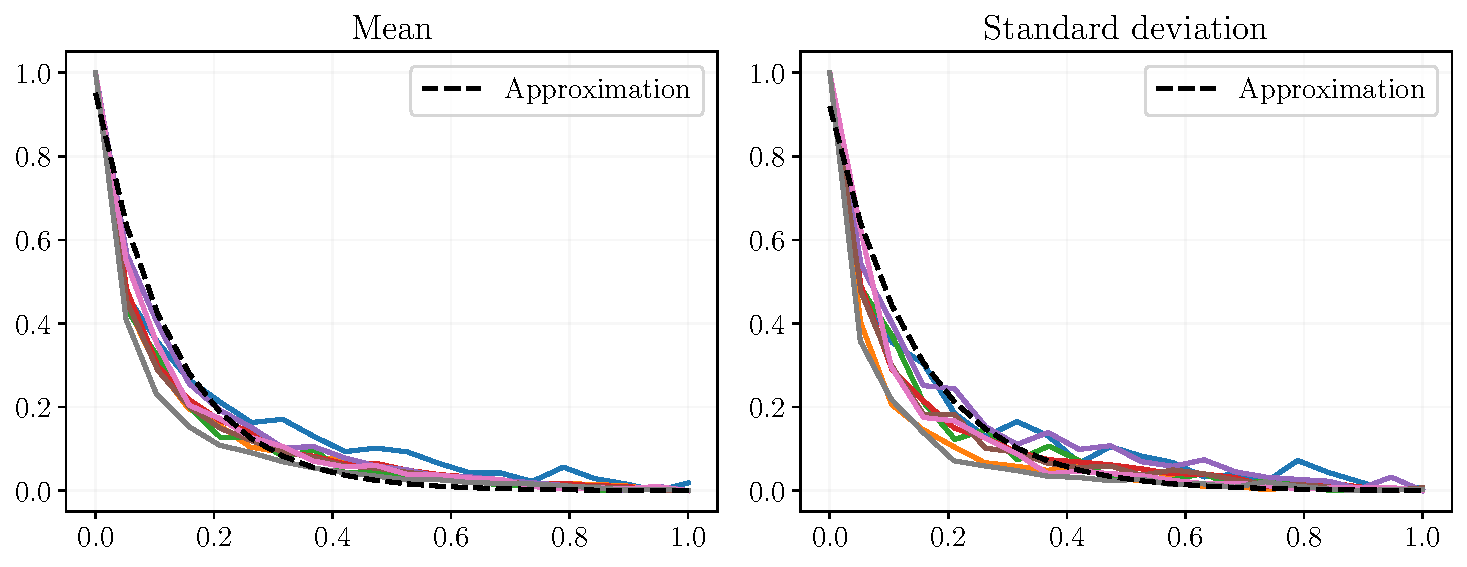
\includegraphics[width=\textwidth]{datasets-regression}
    \caption{Поведение функции ошибки в задаче регрессии}
    \label{datasets-regression}
\end{figure}

Применение генетического алгоритма приводит к одинаковому семейству функций для аппроксимации среднего и среднеквадратичного отклонения в задаче регрессии:
\[ w_0 + w_1 \cdot \exp(w_2 \cdot x). \]

В задаче классификации использовалось 12 датасетов из \citep{UCI}: Automobile, Breast Cancer Wisconsin (Diagnostic), Car Evaluation, Credit Approval, Glass Identification, Ionosphere, Iris, Tic-Tac-Toe Endgame, Congressional Voting Records, Wine, Zoo и Heart failure clinical records. Задача классификации для каждого из них решалась с помощью логистической регрессии из \citep{scikit-learn}. Усреднение производилось по $B = 100$ бутстрап-выборкам. Все завимисости также приводятся к одинаковому масштабу по обеим осям. Полученные графики представлены на Рис.~\ref{datasets-classification}. Как и ранее, слева находится график для выборочного среднего, справа находится график для выборочного среднеквадратичного отклонения.

\begin{figure}[h!]
    \centering
    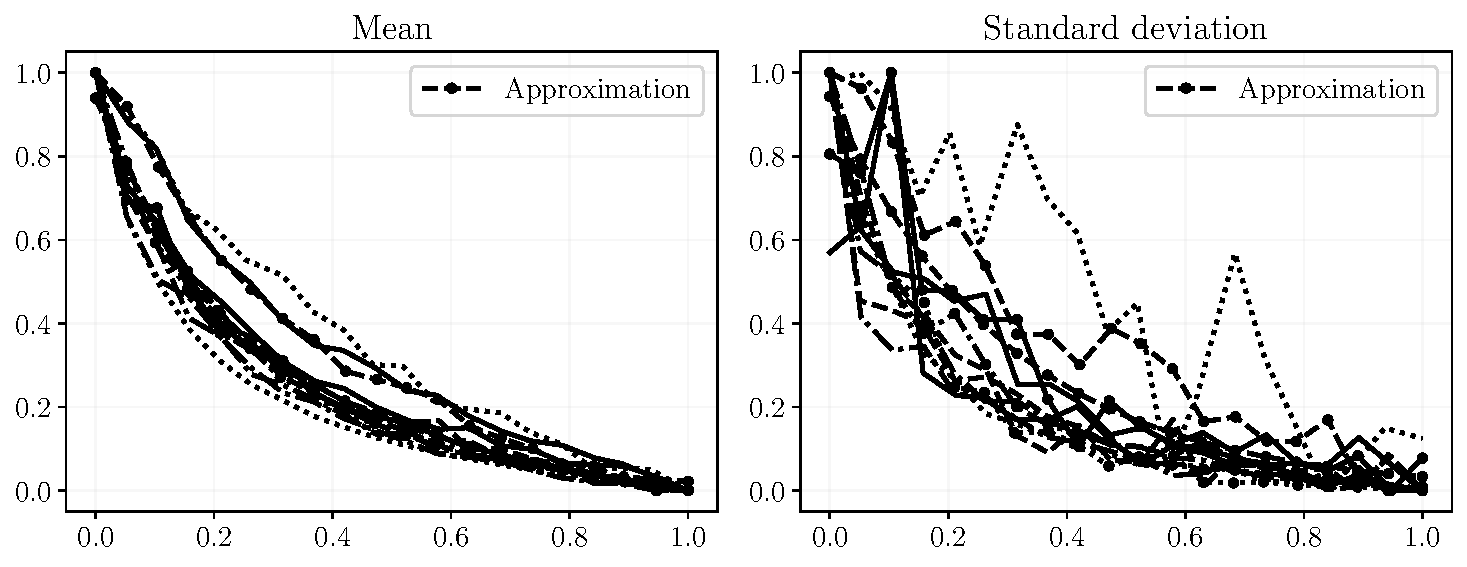
\includegraphics[width=\textwidth]{datasets-classification}
    \caption{Поведение функции ошибки в задаче классификации}
    \label{datasets-classification}
\end{figure}

Применение генетического алгоритма для среднего значения приводит к такому же семейству функций, как и в задаче регрессии:
\[ w_0 + w_1 \cdot \exp(w_2 \cdot x). \]

Среднеквадратичное отклонение в случае задачи классификации для каждой выборки имеет свою зависимость от размера выборки. Таким образом, прогнозировать дисперсию для классификации оказывается достаточно сложной задачей.

\subsubsection{Прогнозирование функции правдоподобия}

Для синтетических выборок проведена аппроксимация функций правдоподобия. Среднее значение и дисперсия аппроксимированы параметрическим семейством функций, приведенным в предыдущем пункте.

Производилось разделение на обучающую и тестовую выборки в соотношении 70:30. Аппроксимация производилась только на обучающей части. Достаточный размер выборки находился в тестовой части. На Рис.~\ref{synthetic-regression-approximation} и Рис.~\ref{synthetic-classification-approximation} представлены истинные и восстановленные зависимости для синтетических данных. Там же указаны определенные по истинной зависимости D-достаточный и M-достаточный размеры выборки. 

\begin{figure}[h!]
    \centering
    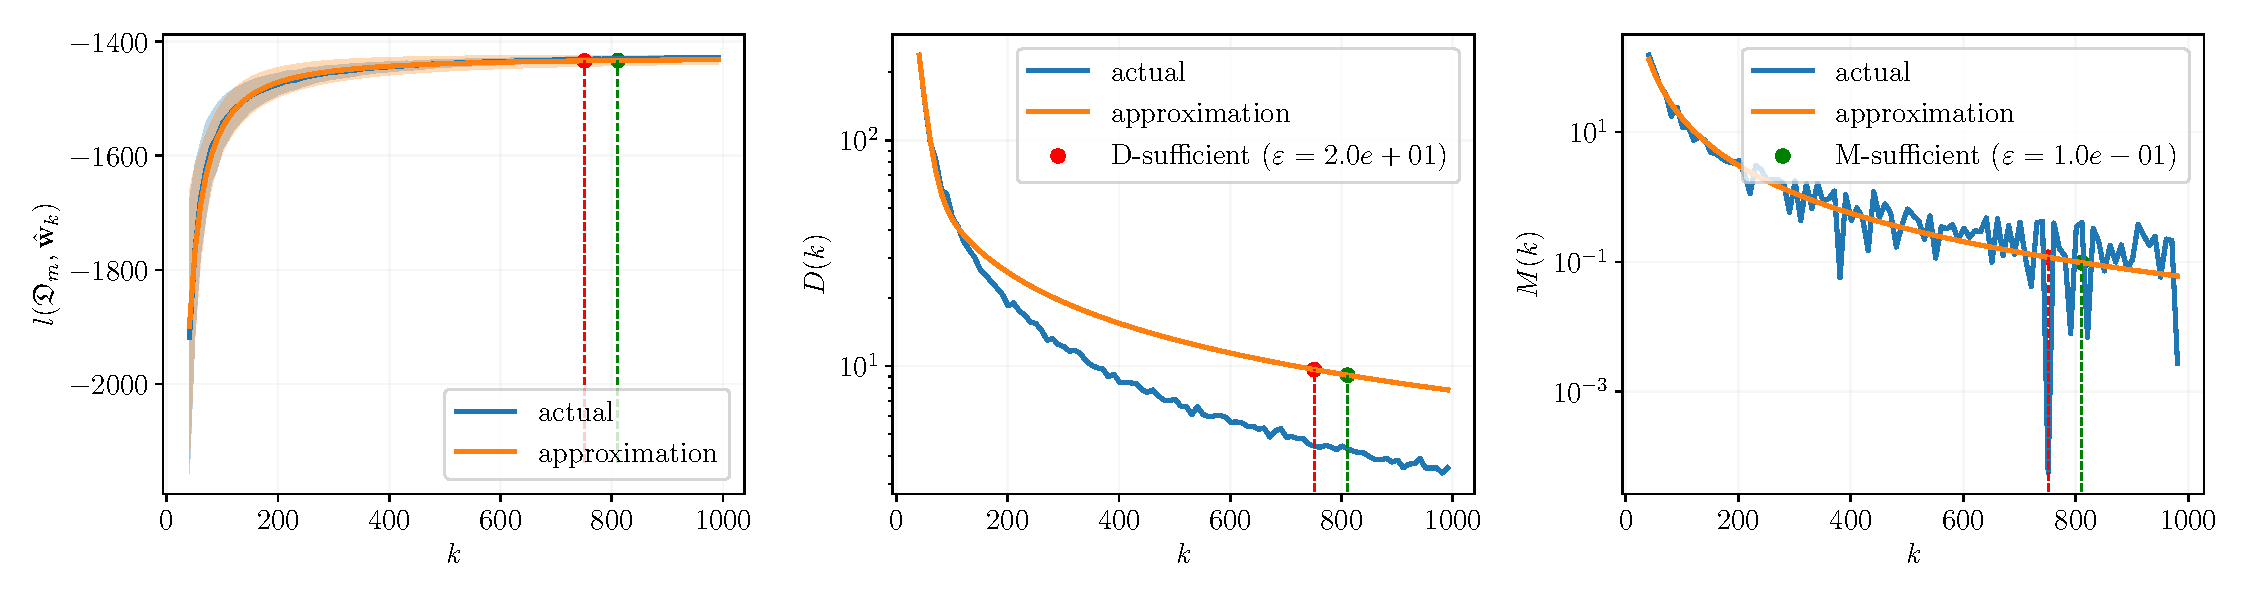
\includegraphics[width=\textwidth]{synthetic-regression-approximation}
    \caption{Синтетическая выборка (линейная регрессия) при $m^* > m$}
    \label{synthetic-regression-approximation}
\end{figure}

\begin{figure}[h!]
    \centering
    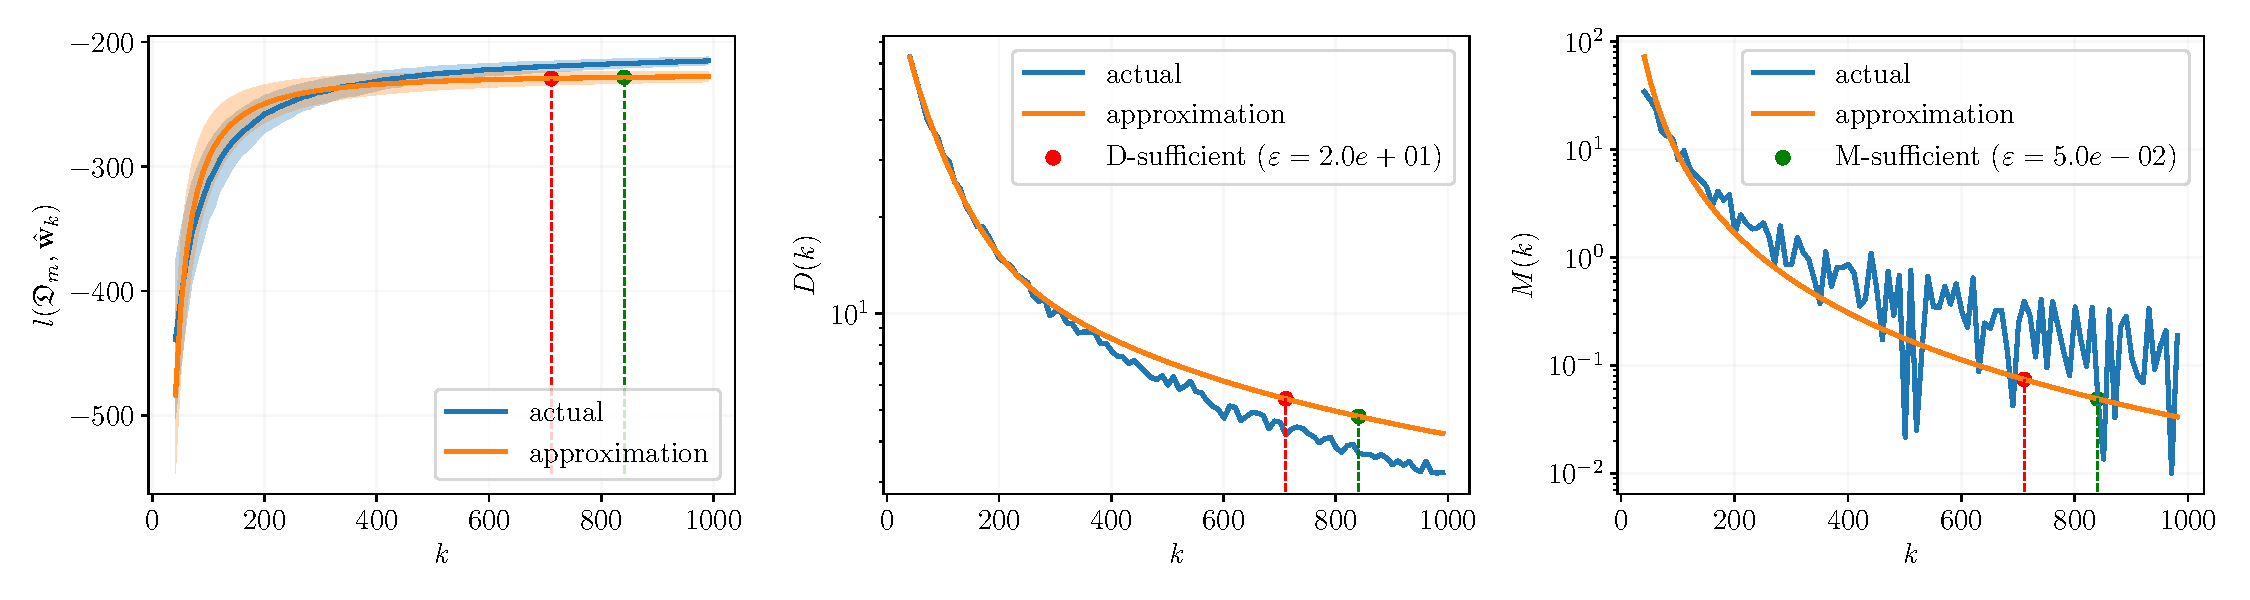
\includegraphics[width=\textwidth]{synthetic-classification-approximation}
    \caption{Синтетическая выборка (логистическая регрессия) при $m^* > m$}
    \label{synthetic-classification-approximation}
\end{figure}

Далее получены аналогичные результаты для выборки Abalone из \citep{UCI}. Они представлены на Рис.~\ref{abalone-approximation}.

\begin{figure}[h!]
    \centering
    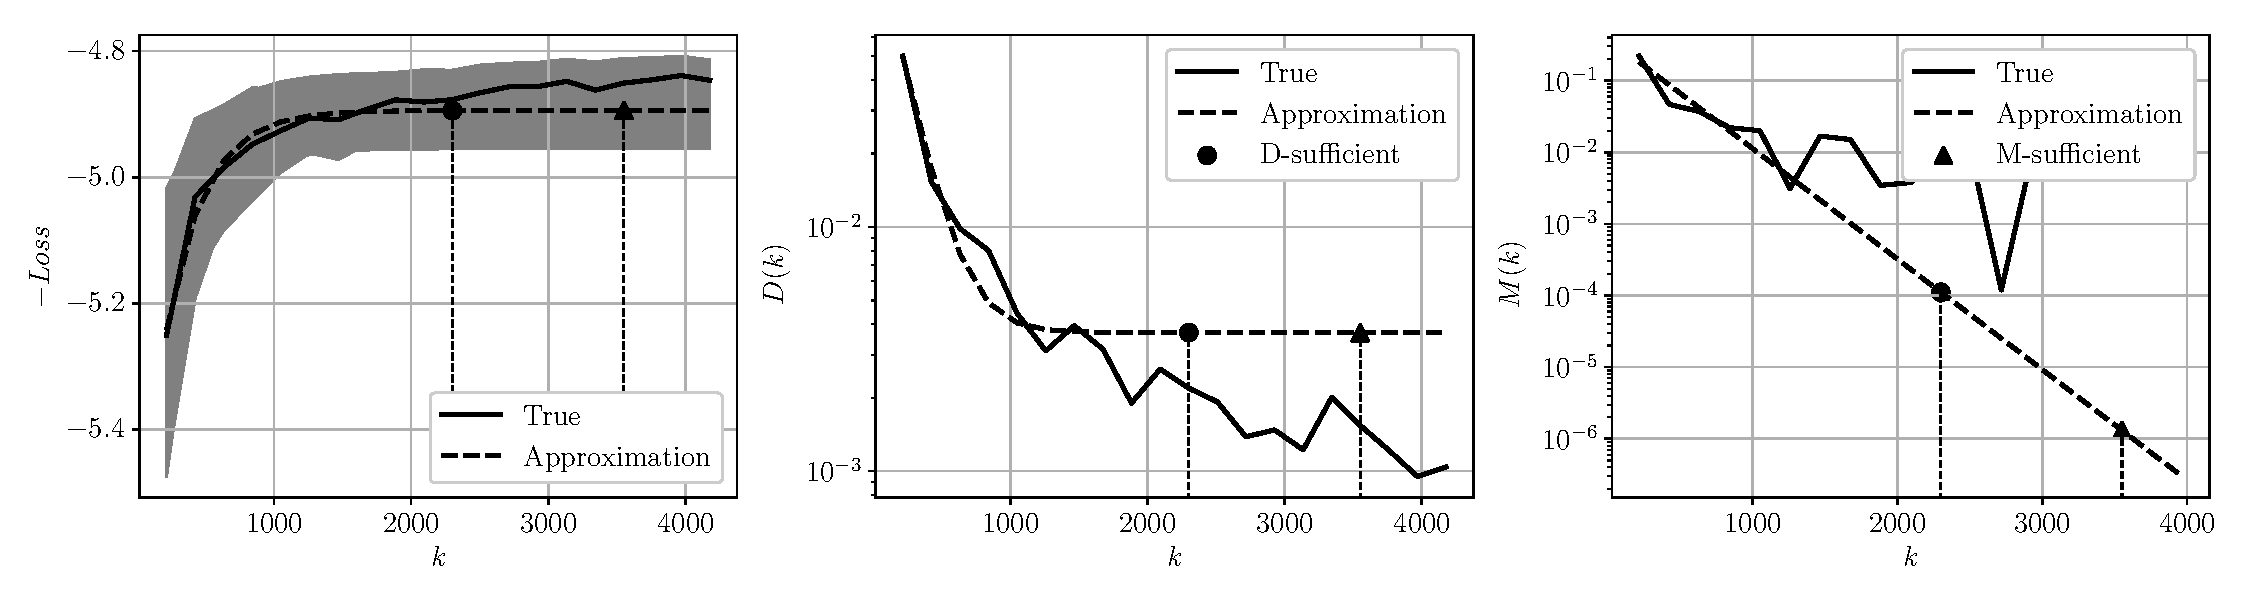
\includegraphics[width=\textwidth]{abalone-approximation}
    \caption{Выборка Abalone (регрессия) при $m^* > m$}
    \label{abalone-approximation}
\end{figure}